\documentclass[11pt,oneside,noprintercorrection,latin1,utf8]{fst-lille}
% Pour les tables
\usepackage{multirow}
\usepackage[table,xcdraw]{xcolor}
%----------------------------------------------------------------------
%                     Chargement de quelques packages
%----------------------------------------------------------------------

% Si l'on veut produire une version PDF avec distiller ou pdflatex :
%\usepackage{tlhypref}
\usepackage[pdfborder=0 0 0]{fst-lille}

% Pour les images :
\usepackage{graphicx}
% Si on veut des mini-tables des matieres (utiliser minitoc-hyper
% en conjonction avec tlhypref) :
%\usepackage[french]{minitoc}
%\usepackage[french]{minitoc-hyper}

\usepackage[frenchb]{babel}
\usepackage{float}

% Pour les codes
\usepackage{listings}
\lstset{language=python,basicstyle=\small}

\synctex = 1

\usepackage[colorinlistoftodos]{todonotes}
\usepackage{pifont}
\usepackage{ulem}

% Correction José
\newcommand{\jose}[1]{\textcolor{red}{#1}}
%-------------------------------------------------------------------
%  Surcharge de commandes pour les variables et page d'en-téte
%-------------------------------------------------------------------

\makeatletter

%
% les deux commandes suivantes sont entre \makeatletter
% et \makeatother parce qu'elles utilisent des `@'.
%

\renewcommand{\@DFD}{}


\renewcommand{\@NancyIhe@d}{{\UseEntryFont{ThesisFirstPageHead}\noindent
    \centerline{
                    {\setbox0=\hbox{$\raise2.3cm\hbox{\FSTInfoLogo}$}%
                     \ht0=\baselineskip\box0}\hfill
                     }%
    \@TL@cmn@head\\
    \par
    }%
    }


\newcommand\TheseLilleI{\renewcommand{\@ThesisFirstPageHead}{\@NancyIhe@d}%
                         \ThesisDiploma{{\UseEntryFont{ThesisDiploma}%
                              \\[3mm]
            {\UseEntryFont{ThesisSpecialty}( )}}}}

\makeatother

%-------------------------------------------------------------------
%           Corrections pour les imprimantes recto-verso
%                          (A AJUSTER)
%-------------------------------------------------------------------

%\ShiftOddPagesRight{-1mm}
%\ShiftOddPagesDown{2.5mm}
%\ShiftEvenPagesRight{0mm}
%\ShiftEvenPagesDown{0mm} 

%-------------------------------------------------------------------
%                Mise en page
%-------------------------------------------------------------------

%-------------------------------------------------------------------
%                             interligne
%-------------------------------------------------------------------
\renewcommand{\baselinestretch}{1.3}

%-------------------------------------------------------------------
%                             Marges
%-------------------------------------------------------------------

% pour positionner les vraies marges:
%\SetRealMargins{1mm}{1mm}

%-------------------------------------------------------------------
%                             En-tetes
%-------------------------------------------------------------------
%On n'utilise pas les logos
%\DontShowLogos

% Les en-tetes: quelques exemples
%\UppercaseHeadings
%\UnderlineHeadings
%\newcommand\bfheadings[1]{{\bf #1}}
%\FormatHeadingsWith{\bfheadings}
%\FormatHeadingsWith{\uppercase}
%\FormatHeadingsWith{\underline}
\newcommand\upun[1]{\uppercase{\underline{\underline{#1}}}}
\FormatHeadingsWith\upun

\newcommand\itheadings[1]{\textit{#1}}
\FormatHeadingsWith{\itheadings}

% pour avoir un trait sous l'en-tete:
\setlength{\HeadRuleWidth}{0.4pt}

%-------------------------------------------------------------------
%                Chemin d'inclusion des graphiques
%-------------------------------------------------------------------

\graphicspath{{img/}{./}}

%-------------------------------------------------------------------
%                         Les references
%-------------------------------------------------------------------

\NoChapterNumberInRef \NoChapterPrefix

%-------------------------------------------------------------------
%                           Brouillons
%-------------------------------------------------------------------

% ceci ajoute une marque `brouillon' et la date
%\ThesisDraft



\begin{document}
\renewcommand{\labelitemi}{$\bullet$}
\renewcommand{\labelitemii}{$\circ$}
%-------------------------------------------------------------------
%                          Encadrements
%-------------------------------------------------------------------

% encadre les chapitres dans la table des matieres:
% (ces commandes doivent figurer apres \begin{document}

%\FrameChaptersInToc
%\FramePartsInToc


%-------------------------------------------------------------------
%            Reinitialisation de la numerotation des chapitres
%-------------------------------------------------------------------

% Si la commande suivante est presente,
% elle doit figurer APRES \begin{document}
% et avant la premiere commande \part
\ResetChaptersAtParts

%-------------------------------------------------------------------
%               mini-tables des matieres par chapitre
%-------------------------------------------------------------------

% preparer les mini-tables des matieres par chapitre.
% (commande de minitoc.sty)
%\dominitoc

%-------------------------------------------------------------------
%                         Page de titre:
%-------------------------------------------------------------------


\ThesisKind{Rapport de projet}
\ThesisPresentedThe{soutenu le 11/12/2019}
\ThesisTitle{Transfer learning et Few-Shot learning pour la détection d'objets}
\ThesisAuthor{BARCHID Sami et ROUGETET Arnaud}
%\NomDuLaboOuEntreprise{Nom labo ou entreprise}
%\LogoLaboOuEntreprise{alcove} % Image du logo du labo ou ets dans le rep img

\NomDuLaboOuEntreprise{Équipe FOX - CRIStAL}
\LogoLaboOuEntreprise{thumb_logo-FOX.png} % Image du logo du labo ou ets dans le rep img TODO

\TheseLilleI

\NewJuryCategory{encadrant}{\it Encadrant : MENNESSON José}
                        {\it Encadrant : TIRILLY Pierre}

%\encadrant = {Nom encadrant 1\\
%              Nom encadrant 2}

% Creation de la page de titre:
\MakeThesisTitlePage

%-------------------------------------------------------------------
%                  ecriture de `Chapitre' et `Partie'
%                      dans la table des matieres
%-------------------------------------------------------------------

\WritePartLabelInToc \WriteChapterLabelInToc

% ABSTRACT %
\SpecialSection{Abstract}

La détection d'objets via l'utilisation du deep learning permet actuellement d'obtenir les meilleurs résultats en terme de précision. Mais de tels détecteurs ont besoin d'être entraînés à partir d'une très grande quantité d'images annotées alors que cette étape d'annotation de données est très coûteuse en terme de moyens. Cependant, l'entraînement de détecteurs à partir d'une quantité limitée d'images reste un problème ouvert dans le domaine. Pour le résoudre, les approches de transfer learning (TL) et de few-shot object detection (FSOD) font partie des solutions envisagées. 

Dans ce rapport, nous conduisons un état de l'art sur ces deux approches. Nous établissons le contexte d'utilisation et une catégorisation propre pour chacune des deux méthodes. Nous comparons ensuite les résultats des modèles constituant l'état de l'art afin de fournir, pour chaque méthode, une base de discussion concernant ses avantages et inconvénients. Nous voyons, à travers ce document, les limitations actuelles de ces méthodes et tentons de comprendre comment les améliorer. Finalement, nous décrivons le travail pratique que nous mènerons ultérieurement et dont le but est d'apporter une comparaison des algorithmes de détection constituant l'état de l'art du transfer learning et de la few-shot object detection.

%-------------------------------------------------------------------
%                        table des matieres
%-------------------------------------------------------------------

\tableofcontents

%-------------------------------------------------------------------
%              Exemple d'utilisation de \SpecialSection
%-------------------------------------------------------------------

% La commande \mainmatter (nouvelle commande LaTeX2e) permet de passer
% a la numerotation arabe (ce que fait \pagenumbering{arabic})
% et de faire commencer la nouvelle page 1 sur une page impaire.
% On evitera donc d'utiliser directement \pagenumbering{arabic}.
\mainmatter

% ----------------------------------------------------------------

% Introduction %
\SpecialSection{Introduction}
\label{chap:introduction}
% Pour ne pas avoir le mot `Chapitre' au debut de chaque chapitre. 
\NoChapterHead
La détection d'objets est une des tâches de vision artificielle les plus étudiées par la communauté scientifique dû à l'étendue des applications pratiques qu'elle permet (voitures autonomes, vidéo-surveillance, etc). Des progrès significatifs ont été faits ces dernières années grâce à l'apparition des techniques de deep-learning en vision par ordinateur. De nos jours, les algorithmes de détection à base de réseaux de neurones \cite{Object-detection-survey} sont devenus la référence dans la communauté grâce à la précision qu'ils offrent.

Comme les techniques de deep learning font partie de la catégorie des algorithmes d'apprentissage supervisé, les détecteurs à base de réseaux de neurones ont logiquement besoin d'images annotées manuellement pour fonctionner. Ils ont généralement besoin d'un très grand nombre de ces données annotées, malgré le fait que celles-ci soient coûteuses en terme de moyens \cite{Su2012CrowdsourcingAF}.

Pour répondre à ce problème, plusieurs pistes sont explorées par la communauté. Nous pouvons par exemple citer la génération d'images synthétiques permettant de construire des données annotées sans effort \cite{DBLP:journals/corr/RajpuraHB17, Baimukashev2019DeepLB}. Parmi ces pistes explorées, deux nous intéressent : la piste du "transfer learning" (TL) \cite{deep-tl} et la piste de la "few-shot object detection" (FSOD) \cite{FSL-survey}. La première consiste à "transférer" le savoir d'un réseau de neurones vers un autre pour que ce dernier ne doive plus apprendre à partir de zéro. La piste de la FSOD consiste à rendre capable un détecteur de pratiquer une détection sur base d'un petit nombre fixé d'images annotées.

Dans le cadre de notre Master 2 spécialité "Image Vision Interaction" (IVI) au sein de l'Université de Lille, nous devons travailler sur un projet scientifique (PJS) visant à réaliser un travail de recherche sur un sujet en lien avec les thèmes abordés par la spécialisation. C'est dans cette optique-là que nous avons décidé de participer à un travail de recherche destiné à explorer le transfer learning et la FSOD. Nous travaillons sous la supervision de José MENNESSON et Pierre TIRILLY, au sein de l'équipe FOX \footnote{\href{http://www.cristal.univ-lille.fr/FOX/}{Fouille et indexation de dOcuments compleXes et multimedia}} du laboratoire CRIStAL.

Dans ce rapport, nous discutons de notre recherche bibliographique sur ces deux sujets. Nous commençons par placer les bases théoriques des réseaux de neurones nécessaires à la compréhension des techniques de deep learning qui sont utilisées en vision artificielle. Ensuite, nous enchaînons par la mise en contexte des tâches de vision artificielle discutées pendant ce rapport et de l'impact du deep learning sur ces tâches. Nous présentons, par la suite, les approches de transfer learning puis de la few-shot object detection en synthétisant notre bibliographie réalisée sur l'état de l'art de ces deux approches. Après cela, nous tentons de réaliser une analyse et une critique des résultats publiés par la littérature scientifique. Enfin, nous terminons en décrivant le travail pratique qui va suivre ce rapport de bibliographie.

%--------------------------------------------------------------------------------------
%--------------------------------------------------------------------------------------

% Deep learning en vision artificielle %
\chapter{Le deep learning pour la vision artificielle}
\label{chap:deep-learning}
Nous nous intéressons ici au deep learning dans le cadre d'un apprentissage supervisé. Le but d'un réseau de neurones est de faire correspondre une base de données d'entrée (dans notre étude, des images) à une base de données de sortie (qui peut être des labels, une nouvelle image générée, une bounding box ou un pourcentage d'appartenance à une image). Le réseau ainsi construit peut être vu comme une fonction résolvant un problème particulier. Les deux types de réseaux sont les réseaux résolvant des problèmes de classification (catégoriser les entrées selon des valeurs discrètes correspondant à des classes définies) et ceux résolvant des problèmes de régression (évaluer des valeurs continues de sortie en fonction des valeurs d'entrée).

\section{Fonctionnement d'un neurone}
\label{sec:neurone}

Un \textit{neurone} est une entité informatique qui prend un vecteur de valeurs $\textbf{x} = (x_1, x_2, ..., x_d)$ en entrée pour retourner une valeur $y$ en sortie. Chaque $x_i$ est associé à un poids $w_i$ initialisé aléatoirement au départ. À l'intérieur du neurone, deux opérations sont exécutées. La première est la fonction de transfert $\Sigma = b + \sum{x_i \cdot w_i}$ où $b$ est une valeur nommée "biais". La deuxième est une fonction non-linéaire $f$ nommée "fonction d'activation" qui prend le résultat de la fonction de transfert en paramètre et retourne la sortie $y$. La figure \ref{fig:schema-neurone} illustre l'organisation d'un neurone. On peut résumer un neurone par l'équation suivante :
\begin{equation}
    y = f(\Sigma) = f(b + \sum_i{x_i \cdot w_i})
\end{equation}

\begin{figure}[!h]
\centering
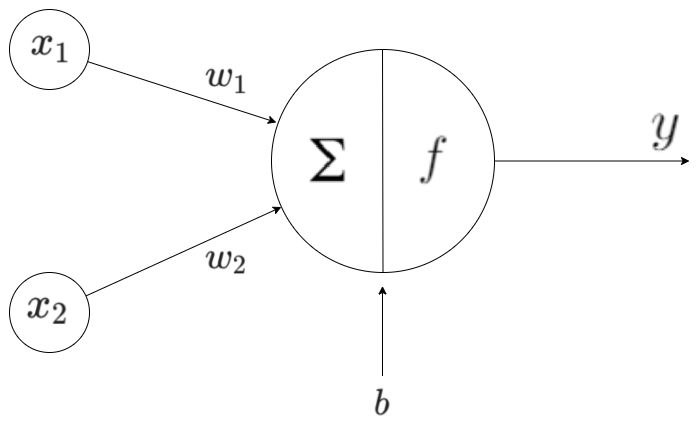
\includegraphics[scale=0.5]{img/neurone.PNG}
\caption{Schéma d'un neurone à deux entrées.}
\label{fig:schema-neurone}
\end{figure}

\section{Fonctionnement d'un réseau de neurones}
Plusieurs neurones connectés entre eux forment un \textit{réseau de neurones} (figure \ref{fig:exemple_network}). Les neurones sont regroupés par \textit{couches}. La première couche est appelée \textit{couche d'entrée}. Elle représente les valeurs que l'on fournit en entrée au réseau\footnote{Cette première couche n'effectue aucun calcul et se contente de passer les entrées à la couche suivante.}. La dernière couche est appelée \textit{couche de sortie}. Les résultats de cette couche sont les résultats finaux. Les autres couches sont les \textit{couches cachées}.

\begin{figure}[!h]
\centering
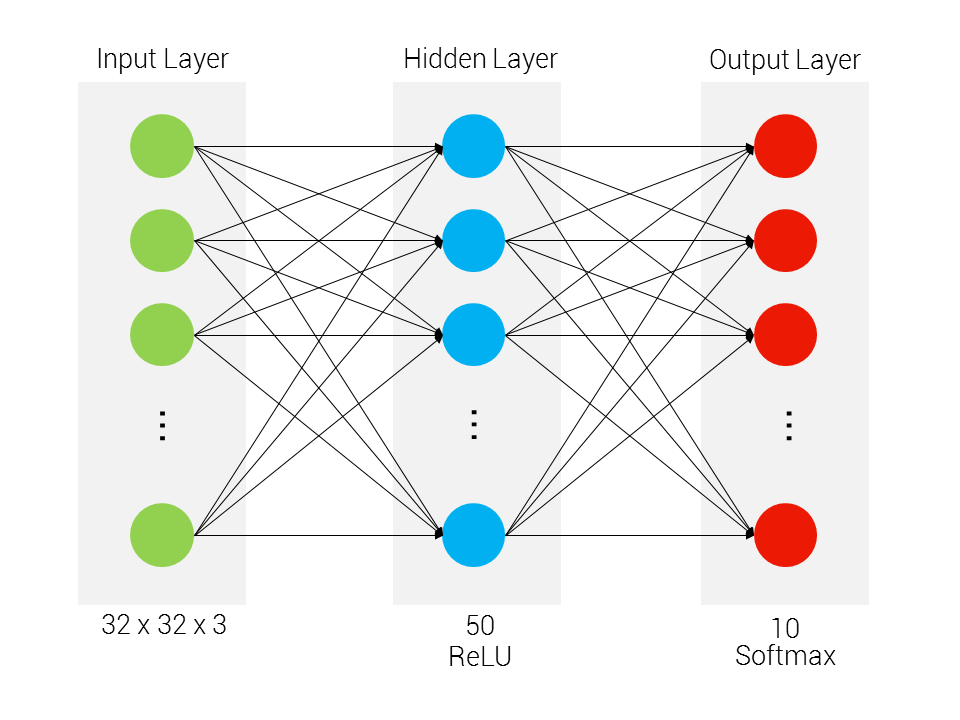
\includegraphics[scale=0.5]{img/neural_ex.png}
\caption{Exemple d'un réseau de neurones avec une couche d'entrée, une couche de sortie et une couche cachée. Source :  \url{https://ljvmiranda921.github.io/notebook/2017/02/17/artificial-neural-networks/}}
\label{fig:exemple_network}
\end{figure}

À l'initialisation, les poids et les biais des neurones sont choisis aléatoirement. L'ensemble des poids et des biais utilisés dans un réseau de neurones est noté $\theta$. Le but est de changer $\theta$ afin que le réseau fasse correspondre les entrées aux sorties. Cette phase de changement des paramètres s'appelle \textit{"phase d'entraînement"}. On utilise généralement une grande quantité de données annotées pour cette phase.

Pour entraîner un réseau, on effectue les tâches suivantes :
\begin{itemize}
  \item On entre des données dans le réseau par la couche d'entrée.
  \item On calcule  la "fonction de coût"\footnote{Loss, en anglais.}, qui permet d'évaluer la différence entre les sorties du réseau de neurones et ce qui était attendu.
  \item On utilise une "fonction d'optimisation" (par exemple, la descente du gradient) qui permet de corriger petit à petit les poids pour minimiser la fonction de coût, grâce à la \textit{rétro-propagation} ("backpropagation", en anglais) de la fonction de coût.
\end{itemize}

% TODO
La \textit{backpropagation} consiste à appliquer une fonction qui propage l'erreur entre la prédiction et le résultat attendu. Les poids de chaque couche et des liens sont corrigés en partant de la couche de sortie puis en remontant jusqu'à la couche d'entrée.

\section{Réseau de neurones convolutionnel}

\begin{figure}[!h]
\centering
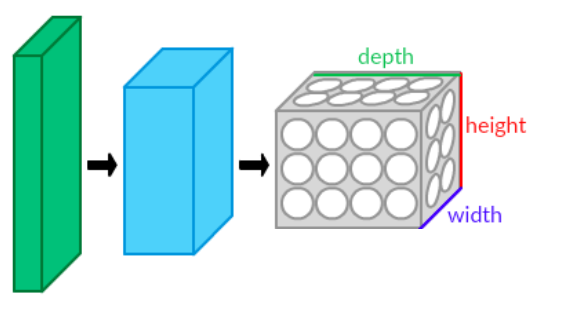
\includegraphics[scale=0.4]{img/Conv_layers.png}
\caption{Illustration d'une couche de convolution d'un CNN. La couche verte montre le volume des entrées, la couche bleue montre la couche de neurones construite en filtres de convolution (avec une profondeur). Après la convolution du volume d'entrée par la couche de convolution, on obtient le volume de sortie, en gris, dont la largeur, la hauter et la profondeur ont été modifiées. Source : \url{https://www.wikiwand.com/fr/R\%C3\%A9seau_neuronal_convolutif}}
\label{fig:cnn-layer}
\end{figure}

Les réseaux de neurones classiques fonctionnent mal en vision artificielle, pour la raison que les données en entrée sont des images, c'est-à-dire des tenseurs de $W \times H \times 3$ pixels pour des images couleurs RGB de largeur $W$ et de hauteur $H$, par exemple. Un réseau de neurones classique ne permet pas de retenir la notion de structure géométrique des pixels dans une image, ce qui aboutit à des performances peu convaincantes en vision artificielle.

Les réseaux de neurones convolutionnels (CNN\footnote{Convolutional Neural Network}, en abrégé) sont une variante des réseaux de neurones qui permettent de répondre à ce problème et qui sont la brique de base des solutions de deep learning en vision par ordinateur. Les CNNs sont composés de \textit{couches de convolutions}, des couches où les neurones sont organisés à la manière de filtres de convolutions sur les données d'entrée. La figure \ref{fig:cnn-layer} illustre brièvement le fonctionnement d'une couche de convolution.

Des recherches \cite{CNN-visu} ont montré que ces couches de convolution permettent de calculer et récupérer des caractéristiques de l'image. Les premières couches de convolution retirent des caractéristiques bas-niveau (contours, par exemple) tandis que les couches plus profondes sont sensibles à des caractéristiques plus haut-niveau. La figure \ref{fig:features-cnn} illustre l'apprentissage de ces caractéristiques en fonction de la profondeur des couches.

\begin{figure}[!h]
\centering
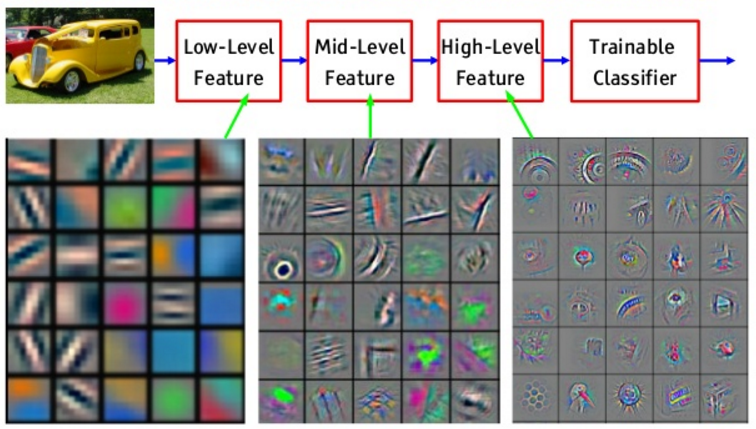
\includegraphics[scale=0.4]{img/cnn-vizzzz.png}
\caption{Illustration des caractéristiques de l'image extraites par un CNN. Des caractéristiques bas-niveau comme des contours sont extraites dans les couches les moins profondes. Puis, des caractéristiques de plus en plus haut niveau sont apprises au fur et à mesure que les couches sont profondes. Source : \url{https://medium.com/@kalfasyan/my-connectionist-approach-to-deep-learning-part-1-a9b190356295}}
\label{fig:features-cnn}
\end{figure}

\section{Définition d'un ensemble de données pour réseau de neurones}
En général, l'ensemble de données (ou "dataset", en anglais) qui traite un problème de vision artificielle contient :
\begin{itemize}
    \item \textbf{Ensemble d'apprentissage :} de nombreuses images supervisées, annotées à la main. Cet ensemble est destiné à faire apprendre au modèle.
    
    \item \textbf{Ensemble de test :} un ensemble (plus petit que l'ensemble d'apprentissage) d'images supervisées. Ces images vont servir à mesurer les performances du réseau après que celui-ci ait été entraîné sur l'ensemble d'apprentissage.
\end{itemize}

\hspace{1pt}
\par\noindent\rule{\textwidth}{0.4pt}
 
Ce chapitre permet au lecteur de prendre connaissance des bases des réseaux de neurones dont nous nous servons dans ce rapport. Ce sont ces bases qui sont, encore aujourd'hui, les fondations de l'application du deep learning dans les tâches de vision par ordinateur. Nous voyons dans le chapitre suivant comment ce principe du deep learning est exploité pour résoudre les tâches de vision artificielle rencontrées dans ce projet.

% Travaux liés
\chapter{Le deep learning en vision artificielle}
\label{chap:related-works}
Dans ce chapitre, nous décrivons les notions nécessaires de vision par ordinateur pour placer le contexte de notre travail. Nous faisons ensuite le lien entre l'utilisation du deep learning pour résoudre ces tâches et les nouvelles problématiques engendrées par cette utilisation.

% Classification d'image
\section{Classification d'images vs détection d'objets}
\label{sec:class-vs-detect}
Parmi les tâches de vision artificielle existantes, deux d'entre elles sont très populaires et ont de nombreuses applications. Ces deux techniques sont la classification d'images et la détection d'objets. Nous nous intéressons dans ce rapport à la détection, mais il est important pour la suite de comprendre également ce qu'est la classification.

\subsection*{Classification d'images}
Un algorithme de classification d'images \cite{classification-survey} prend une image en entrée dans le but de fournir une classe ou des probabilités d'appartenir à une classe en sortie. Les modèles de classification analysent les caractéristiques de l'entièreté de l'image afin de déterminer la classe. C'est pourquoi, habituellement, les images utilisées pour la classification présentent un seul objet à reconnaître en avant-plan avec un arrière-plan peu encombré. En générale, les performances d'un modèle de classification d'images sont mesurées via un taux de bonne reconnaissance sur les images de test d'un dataset.

\subsection*{Détection d'objets}
Un algorithme de détection \cite{Object-detection-survey} prend une image en entrée, détecte les instances des objets recherchés et fournit en sortie, pour chacun d'eux, une localisation au moyen d'une \textit{bounding box}\footnote{Boite englobante, en français.}. On peut citer comme exemple d'applications pratiques : la détection de défaut dans une texture \cite{7966162} ou encore la position d'objets dans une vitrine \cite{Sun2019ExploringBF}. Contrairement au problème de classification, la détection est un problème de régression. Il y a plusieurs difficultés en détection. Tout d'abord il faut analyser les caractéristiques de parties de l'image où peuvent se trouver une ou plusieurs instances d'objets recherchés. Et, ensuite, il faut fournir une bounding box placée de la manière la plus précise possible autour d'un objet détecté.


\begin{figure}[!h]
\centering
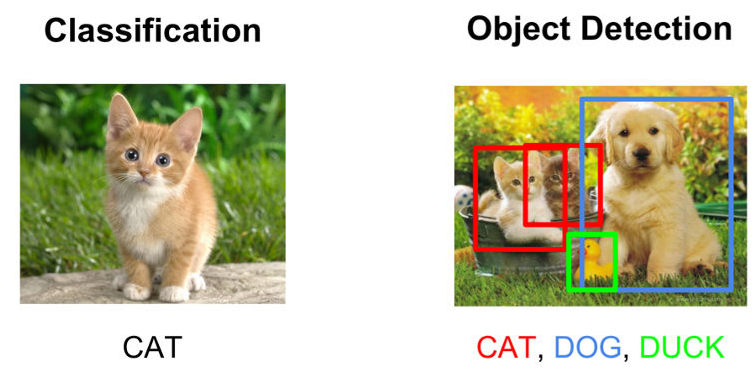
\includegraphics[scale=0.5]{img/Classi-vs-detect.PNG}
\caption{Exemple montrant la différence entre la détection et la classification. Source : \url{https://www.datacamp.com/community/tutorials/object-detection-guide}.}
\label{fig:class-vs-detec}
\end{figure}

\subsubsection*{Mesure de la performance d'un détecteur}
Les images d'apprentissage annotées, disponibles dans les datasets de détection, sont déjà munies de bounding boxes. Celles-ci sont connues sous le nom de "vérité terrain"\footnote{"ground truth", en anglais.}. Ainsi, pour quantifier la performance d'un détecteur, on utilise une mesure qui compare les bounding boxes trouvées à la vérité terrain. En général, les algorithmes de détection utilisent le \textit{mAP}\footnote{Mean Average Precision} \cite{hui_2018} pour mesurer la performance de la détection. En résumé, la mAP mesure la moyenne des surfaces des bounding boxes trouvées par le détecteur par rapport aux bounding boxes de la vérité terrain sur toutes les images et en tire un pourcentage.

\section{Détection d'objets et deep learning}
Avec le succès du deep learning en classification d'image \cite{im-class-nn}, les algorithmes de détection sur base du deep learning ont aussi eu une belle évolution. On peut classer les algorithmes de deep learning pour la détection d'objets en deux catégories :
\begin{itemize}
    \item \textbf{Détecteurs two-stage} \cite{R-CNN, Fast-RCNN, Faster-R-CNN} : ces algorithmes opèrent la détection en deux étapes (d'où le nom). Dans un premier temps, le détecteur identifie des régions d'intérêts (ROI\footnote{Region Of Interest}, en abrégé) qui sont susceptibles de contenir une instance d'un objet recherché. Ensuite, un classifieur discrimine ces ROIs pour déterminer si elles contiennent bel et bien un objet. Les détecteurs de type two-stage sont plus lents mais plus précis. Ils ne sont généralement pas adaptés pour du temps réel.
    \item \textbf{Détecteurs one-stage} \cite{YOLO, YOLO9000, YOLOv3, SSD, Retinanet} : ces algorithmes opèrent en une seule étape. Ils opèrent la détection sur un ensemble de localisations selon une grille pré-définie par l'utilisateur . Les détecteurs one-stage sont moins précis mais sont plus rapides. C'est pourquoi ils sont plus adaptés pour du temps réel.
\end{itemize}
Même si les détecteurs à base de deep learning sont actuellement les plus performants en terme de précision, ils ont également introduit un problème au niveau de la quantité d'images annotées manuellement à fournir. On peut voir, par exemple, des problèmes de détection \cite{COCO} avec plus de 330 000 images annotées pour détecter 80 classes d'objets. On peut donc constater que les algorithmes classiques de détection en deep learning requièrent une étape d'annotation manuelle très coûteuse qui peut s'avérer compliquée dans des conditions où on ne dispose pas d'assez de moyens.

% Transfer learning
\section{Transfer learning (TL)}
Une méthode pour pallier au manque d'image est le transfert learning. Le transfer learning consiste à entraîner un réseau de neurones en utilisant deux bases de données. Avec une première base de donnée, appelée la \textit{source}, on va pré-entraîner le réseau. Le but du pré-entraînement est de faire en sorte que le réseau apprenne à faire de l'extraction de caractéristiques sur des images (du type extraction des edges). On va ensuite apporter des modifications au réseau qui vont varier en fonction de l'objectif à atteindre. Enfin, on va entraîner le réseau modifié sur une base de données appelée la \textit{destination}. C'est dans la \textit{destination} que se trouvent les données qui vont nous permettre de résoudre le problème posé.

Dans le principe, la source sera un dataset très grand comme ImageNet \cite{ILSVRC15} avec plusieurs millions d'images qui permettra un entraînement du réseau avec une très grande efficacité. En effet, un réseau a besoin de beaucoup de données pour apprendre et, plus il a d'image, meilleur sera l'apprentissage. La destination sera, quant à elle, la base considérée qui sera généralement de petite taille. Pour des problèmes pratiques, une base de données de petite taille sera inférieure à 5000 images mais de nombreux travaux de recherche considèrent que des bases de données qui sont inférieures à 20000 images sont aussi de petite taille.

Les modifications doivent permettre de reprendre une partie de l'analyse faite par le réseau sur les données sources que la plupart des travaux supposent être les mêmes ou proches de celles sur les données de destination.

Il existe différentes approches de transfer learning qui prennent en compte l'objectif voulu, le type de réseau utilisé ou les données disponibles.

D'autres techniques prennent en compte le \textbf{type de réseau}. Certaines techniques sont spécifiques aux réseaux les plus grands (les \textit{profonds}) \cite{DBLP:journals/corr/abs-1804-06275} et certains sont même spécialisés pour les réseaux Deep que l'on appelle des "réseaux adverses" \cite{DBLP:journals/corr/CaoL0J17}.

Les techniques de transfer learning qui prennent en compte les \textbf{bases de données} sont des techniques qui vont s'appuyer sur le nombre d'images dans la destination \cite{Sun_2019_CVPR}, les différences entre la base source et destination et le fait que l'on puisse avoir plusieurs sources ou plusieurs destinations \cite{Dwivedi_2019_CVPR}. C'est ce genre d'approche qui a donné lieu au développement du \textbf{Few-Shot learning}, qui est une approche que nous détaillons dans le chapitre \ref{chap:FSOD}.

\hspace{1pt}
\par\noindent\rule{\textwidth}{0.4pt}

Les problèmes liés à l'utilisation du deep learning en vision artificielle décrits dans ce chapitre montrent le besoin de développer de nouvelles techniques, notamment pour réduire le nombre d'images à annoter à la main à fournir pour entraîner ces réseaux. Nous introduisons deux approches pour régler ce problème : le transfer learning et le few-shot learning. Dans la suite du rapport, nous décrivons ces deux approches et synthétisons les méthodes récentes dans ces domaines.

% Transfer learning %
\chapter{Transfer learning}
\label{chap:transfer-learning}

Les approches du transfer Learning (TL) sont nombreuses. Cependant, les premières techniques de TL faisaient hypothèse qu'il existe un lien entre les images de la source et celles de la destination. Cela pouvait être une similarité de classe, par exemple de la salade en sources et des soupes en destination qui sont tout deux de la nourriture, ou des caractéristiques communes. Par exemple, des vélos en sources et des trottinettes en destination qui ont tout deux des roues.

L'idée étant que certaines couches contiennent en elles l'extraction et l'identification de ces caractéristique, le but est d'exploiter au mieux ces couches afin de pouvoir entraîner plus rapidement ou plus efficacement un modèle pour une nouvelle tâche.

Chaque spécialisation de transfer learning va donc correspondre à un enjeux bien particulier.

\section{Multi-data Transfer Learning}
\label{sec:multi-data}
Afin de pallier le problème du manque de données, une approche est de multiplier les bases de données afin de profiter de l'apprentissage de certaines caractéristiques dans le réseau, soit en profitant de plusieurs sources, soit en exploitant les similarités d'un même apprentissage sur différents domaines.

\subsection{Multi-sources TL}
\label{subsec:multi-sources}

Le Multi-source Transfer Learning \cite{multi-source} est une méthode qui consiste à essayer d'effacer les différences de caractéristiques entre le domaine source et une destination en multipliant les sources. On va donc disposer, avec ce genre de méthodes, de $N$ sources avec lesquelles on va entraîner $N$ réseaux. Chaque réseau va disposer de couches extractrices de caractéristiques et de couches classifieurs. Dans le réseau final, les $N$ couches d'extractions sont rassemblées ensemble et on fait de même avec les couches de classifications.

Ensuite, une fois que l'on a obtenu ce réseau final, il va être entraîné avec les données de destination de manière classique.

\subsection{Multi-tasking Learning}
\label{subsec:multi-tasking}

Le multi-tasking Learning est une méthode qui consiste à appliquer plusieurs traitements à une même image. Par exemple, segmenter l'image en fonction des profondeurs ou générer l'image des normales. Du fait que l'on parte d'une même source pour ces images, on va pouvoir calculer la similarité entre une tâche et les autres. Les réseaux des différentes tâches vont être séparés mais vont prendre en compte des éléments des autres réseaux dans leur fonction de coût et leur fonction d'optimisation.

L'apprentissage est ainsi réparti entre chaque réseau tout en faisant en sorte que chaque réseau soit spécialisé dans une seule tâche.

La méthode de multi-tasking la plus complète est celle de Stanford appelé "Taskonomie" \cite{tasknomie-presentation}. Le score de similarité entre tâches est calculé à partir d'une méthode inspirée des neurosciences appelées RSA (Representation Similarity Analysis). Il est créé une matrice des similarités qui donne une vue globale des correspondances entre chaque tâche et les autres. La matrice est le résultat de l'application directe du calcul RSA entre chaque couple de base de données. Les fonctions de coût des réseaux des $N$ tâches vont prendre en compte la matrice de similarité. Ainsi, chaque tâche va prendre en compte la progression d'une tâche qui est proche d'elle.

Cela nécessite plus de contraintes sur les données que le multi-source car toutes les destinations doivent être liées à la même source. La base de données la plus complète que nous avons trouvée est celle de Stanford qui propose 15 destinations pour une même source \cite{zamir2018taskonomy}.

Cependant cette méthode ne réduit pas le nombre de données par tâche. Par contre, l'entraînement commun permet une convergence plus rapide et un taux de réussite plus grand que si les tâches sont entraînées individuellement.


\section{Deep Learning Transfer}
\label{sec:deepT}

Les travaux catégorisés en tant que "Deep Learning en TL" sont les travaux qui vont se focaliser sur un réseau en particulier (resnet, YOLO, etc) ou un réseau et une tâche particulière et expliquer quelles sont les couches à enlever/modifier ou les fonctions de coût optimum à utiliser avec ce réseau.

Les réseaux Deep étant actuellement beaucoup utilisés, de nombreux articles \cite{Sun2019ExploringBF, DBLP:journals/corr/abs-1804-06275, 8729686, 7966162} sont basés sur ces approches et cherchent à optimiser leurs résultats par rapport à ceux de travaux déjà existants sur des problèmes similaires. Comme dit précédemment, l'optimisation peut porter sur les couches à remplacer ou ajouter, la fonction de coût ou d'optimisation mais aussi sur la base de données source à utiliser.

Comme on peut le voir sur la figure \ref{fig:features-extract}, les couches basses (proches de l'entrée), vont contenir des données de bas niveau, généralement du filtrage ou de l'extraction de contours. Les couches suivantes vont avoir tendance à se spécialiser dans l'extraction de donner liées aux images fournies. Par exemple, pour la reconnaissance de visages, on voit sur la figure \ref{fig:features-extract} que les couches moyennes reconnaissent des parties de visages (nez, bouche, yeux) et les couches de haut niveau des visages en entier. Le but est donc, pour une tâche particulière, d'identifier les couches "génériques" dont on va vouloir se resservir pour un nouvel apprentissage et quelle est la partie du modèle que l'on ne peut pas garder.

\begin{figure}[!h]
\centering
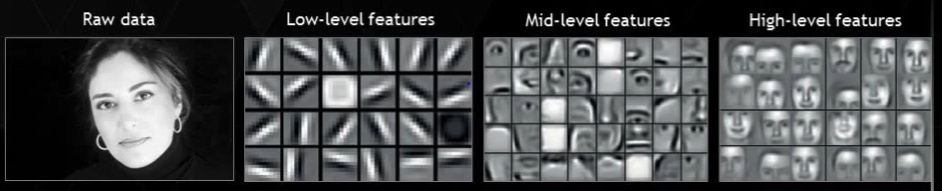
\includegraphics[scale=0.5]{img/features.png}
\caption{Visualisation des descripteurs des couches de bas, moyen et haut niveaux \cite{featureGFaces}}
\label{fig:features-extract}
\end{figure}

Ainsi l'article \cite{Kornblith_2019_CVPR} compare l'efficacité de l'utilisation des bases de données les plus utilisées en tant que source. Les sources les plus utilisées sont ImageNet, COCO, CIFAR et FOOD-101 car elles contiennent plusieurs dizaines de milliers, voire des millions d'images, ce qui les rend intéressantes en tant que sources. Ces sources peuvent, cependant, être éloignées des données de destination. Il est donc nécessaire de faire des tests et de comparer afin de savoir quelles bases de données seront les meilleures pour les cas choisis.

\subsection*{Le cas particulier des réseaux adverses}
\label{subsec:adversials}
Les réseaux deep avec adversial sont un type de réseau particulier. En plus de l'apprentissage d'un réseau profond classique, un deuxième réseau, \textit{l'adversaire} (ou \textit{l'adversial}), est mis à coté du premier et à pour rôle de critiquer l'apprentissage du premier. Le but de cette critique peut être de rendre une classification résistante à des attaques ou de maximiser un critère d'apprentissage précis.

Dans cette optique, des méthodes ont été proposées afin de se servir des réseaux adverses dans le cas du transfer learning et le \textit{Deep Learning Transfer avec Adversial} est une sous-catégorie à part entière du simple \textit{Deep Learning Transfer}.

Le papier le plus intéressant dans cette optique a été celui qui présente les Joint Adaptation Networks (JAN) \cite{DBLP:journals/corr/Long0J16a}, dont l'intérêt et de proposer une version du réseau sans adversaire et une version avec adversaire, appeler JAN-A. Le réseau adverse sert à calculer un critère de minimisation le joint maximum Mean Discrepancy (JMMD). Ce critère représente la distribution conjointe entre la source et la destination. En somme, le but de l'adversaire va être de calculer la distribution conjointe (les points communs) entre les données apprises de la base source et les données de la destination.

Cela permet de récupérer de manière plus efficace sur les caractéristiques communes entre la source et la destination. Le calcul de quelles features garder sera fait directement par le réseau.
Le taux d'apprentissage sur des données ne contenant que 600 images sera équivalent à celui entraîner sur des données en contenant plusieurs milliers.


% Few-shot object detection
\chapter{Few-shot object detection}
\label{chap:FSOD}
Il existe des cas de figures où le manque de données annotées pour un détecteur est poussé à l'extrême. On peut disposer, par exemple, que de moins de 5 images par catégorie d'objets à détecter. La few-shot object detection (FSOD) tente de régler la problématique liée à ce genre de configuration. Dans ce chapitre, nous donnons une formalisation de la FSOD et catégorisons les solutions proposées dans les articles de recherche. Nous explorons aussi les enjeux et les verrous scientifiques présents dans la problématique.


\section{Le few-shot meta-learning dans la classification d'images}
\label{sec:FSOD-FSL-meta}
La problématique que tente de résoudre le few-shot learning se pose aussi dans d'autres techniques de vision artificielle, notamment en classification d'images \cite{FSL-survey} où la communauté travaille sur le sujet depuis plus longtemps que pour la détection d'objets. Nous pensons qu'il est important de placer le contexte du few-shot learning en classification, étant donné que l'état de l'art dans cette technique influence grandement les travaux liés à la FSOD.

\subsection*{Formalisation du problème de few-shot classification}
On parle d'un problème de few-shot classification "$N$-way $K$-shot" pour qualifier le problème où l'on cherche à reconnaître des images de $N$ classes différentes. Pour chacune des $N$ classes, on dispose d'un nombre $K$ réduit d'images supervisées. Habituellement, un problème de few-shot classification se pose sur base d'un nombre d'images $K$ allant de 1 à 10.

\subsection*{Meta-learning en few-shot classification}
Récemment, de grands progrès ont été réalisés en few-shot learning pour la classification \cite{FSL-survey}. Ces progrès sont principalement dus à l'exploitation des méthodes de \textbf{meta-learning}.

Le meta-learning, aussi connu sous le nom de "learning to learn" \footnote{"Apprendre à apprendre", en français.}, est un paradigme qui consiste à faire apprendre à un réseau de neurones à s'adapter le plus rapidement possible à une tâche cible $\textbf{T}$ en se basant sur une "connaissance antérieure" apprise en tentant de résoudre plusieurs tâches d'entraînement $\{\textbf{T}_i\}$. Cette connaissance antérieure se veut assez générale pour permettre au réseau de neurones de s'adapter à des tâches différentes.

Concrètement, en classification d'images, $\textbf{T}$ correspond à la tâche $N$-way $K$-shot de classification d'images recherchée et les tâches $\{\textbf{T}_i\}$ sont d'autres problèmes $N$-way $K$-shot avec lesquelles le modèle apprend à s'adapter plus rapidement à une nouvelle tâche. Les données nécessaires aux tâches $\{\textbf{T}_i\}$ sont reprises de datasets déjà existant\footnote{COCO \cite{COCO}, ImageNet \cite{ILSVRC15}, etc.}. De ce fait, les images des datasets sont reprises, les seules images annotées qui doivent être manuellement produites pour résoudre le problème $N$-way $K$-shot sont celles nécessaires pour $\textbf{T}$.

Le paradigme du meta-learning prend forme de plusieurs manières différentes. Deux variantes nous intéresse pour la suite de ce chapitre :
\begin{itemize}
    \item \textbf{Basé sur le "metric learning"} \cite{prototypical-networks, matching-networks, koch2015siamese, relation-net-fsl} : le modèle réduit l'image en entrée en un vecteur de caractéristiques, d'une dimension inférieure à l'image de base. Ce vecteur est une métrique servant à calculer une distance entre d'autres vecteurs représentant d'autres images. Le modèle apprend donc à calculer une métrique dont la distance entre deux images d'une même classe est minimisée et la distance entre deux images de classes différentes est maximisée. On est alors capable de classer une image sur base de ces distances.
    \item \textbf{Optimisation des paramètres du réseau de neurones} \cite{MAML, Meta-SGD} : le modèle apprend, à l'aide des tâches d'entraînement $\{\textbf{T}_i\}$, à produire une bonne initialisation de ses paramètres (les poids, les meta-paramètres pour la fonction d'optimisation\footnote{Par exemple, le "learning rate" pour la descente de gradient.}, ...) d'une manière à ce qu'il puisse être performant pour résoudre $\textbf{T}$.
\end{itemize}

% Les enjeux
\section{Les enjeux}
\label{sec:FSOD-verrous}
Bien que l'importance de la problématique à laquelle tente de répondre la FSOD est avérée, il n'existe pas encore de méthode efficace et reconnue par la communauté. Ceci est dû aux raisons suivantes, qui sont détaillées dans cette section.

\subsection*{Domaine récent}
\label{subsec:domaine-recent}

La détection d'objets sur base du few-shot learning est un problème qui n'est abordé que depuis très récemment dans la communauté. À notre connaissance, les premiers travaux traitant du sujet ont commencé en 2018 avec \cite{feature-reweighting}. Ce caractère récent de la problématique implique les conséquences suivantes :
\begin{itemize}
    \item Peu d'articles de recherche ont été rédigés pour répondre au problème, ce qui implique qu'il y a encore un nombre de solutions limité à l'heure actuelle.
    \item Les solutions envisagées suivent, pour la majorité, une même tendance mais sont relativement hétérogènes dans leur procédé. Malgré cela, elles montrent des résultats similaires. Il y a encore une difficulté pour identifier une technique précise qui présenterait le meilleur intérêt.
\end{itemize}

\subsection*{Complexité de la détection par rapport à la classification}
\label{subsec:complexite-detection}
Comme évoqué dans la section \ref{sec:FSOD-FSL-meta}, les méthodes de few-shot meta learning en classification parviennent à atteindre des résultats intéressants constituant actuellement l'état de l'art en few-shot classification. Cependant, il est difficile d'appliquer directement les mêmes solutions de few-shot meta-learning en détection d'objets. La détection d'objets est une tâche bien plus complexe que la classification pour deux raisons :
\begin{itemize}
    \item La détection est une tâche qui ne cherche pas uniquement à reconnaître une image mais qui cherche aussi à \textit{localiser} un ou même plusieurs objets.
    \item Les objets à détecter dans une image se trouvent dans des environnements souvent encombrés (\textit{ex. : contenu d'une armoire}) et qui peuvent comporter d'autres objets qui ne sont pas recherchés. Les détecteurs entraînés avec peu de données ont tendance à être trompés par ces objets non-pertinents, qu'ils essaient d'interpréter comme des objets appartenant aux catégories ciblées. La partie du détecteur posant problème est celle qui identifie les zones d'intérêt où pourraient se trouver potentiellement un objet recherché. 
\end{itemize}

La littérature traitant de la FSOD travaille essentiellement sur l'adaptation de ces variantes de meta-learning pour résoudre les soucis liés à la détection.

% Définition problème
\section{Formalisation du problème de FSOD}
\label{sec:FSOD-def-prob}
Dans cette section, nous décrivons de manière formelle le problème rencontré que tente de résoudre un algorithme de FSOD.

On parle de détection d'objets "$N$-way $K$-shot" pour qualifier le problème où le but est d'entraîner un détecteur $\phi$ pour que celui-ci soit capable de détecter dans une image des objets appartenant à $N$ catégories différentes. Pour chacune des $N$ catégories, nous disposons d'un nombre de $K$ images annotées, relativement réduit. Habituellement, un problème de FSOD se pose sur base d'un nombre d'images $K$ allant de 1 à 10. Il faut noter que, dans une même image, il peut y avoir plusieurs fois le même objet ou des objets de plusieurs des $N$ catégories en même temps. Ainsi, il est garanti qu'il existe au moins $K$ instances de chacune des $N$ catégories d'objets dans les données dont on dispose.

Pour régler ce problème, les solutions mises au point partent toutes d'une configuration commune : nous disposons de deux datasets : $D_{support}$ et $D_{query}$. $D_{support}$ comprend un grand nombre d'images déjà labélisées selon un ensemble de classes d'objets $C_{support}$, tandis que $D_{query}$ est composé de peu d'images annotées avec les classes $C_{query}$. En pratique, $D_{support}$ est un dataset déjà existant que l'on divise en tâches d'entraînement $\{\textbf{T}_i\}$ qui correspondent à plusieurs problèmes $N$-way $K$-shot. Les tâches $\{\textbf{T}_i\}$ servent à créer la connaissance antérieure du détecteur, qui sera alors capable de s'adapter pour améliorer sa détection sur la tâche cible $\textbf{T}$. $\textbf{T}$ est le problème $N$-way $K$-shot que le détecteur doit résoudre où les $K$ classes d'objets forment l'ensemble de classe $C_{query}$ et les $N \times K$ images labélisées forment $D_{query}$. La figure \ref{fig:Formalisation-FSOD} illustre cette configuration.

La phase d'apprentissage du détecteur est réalisée grâce aux tâches $\{\textbf{T}_i\}$. Ensuite, le détecteur est optimisé pour $\textbf{T}$ avec les $N \times K$ images disponibles pour $D_{query}$.
\begin{figure}[!h]
\centering
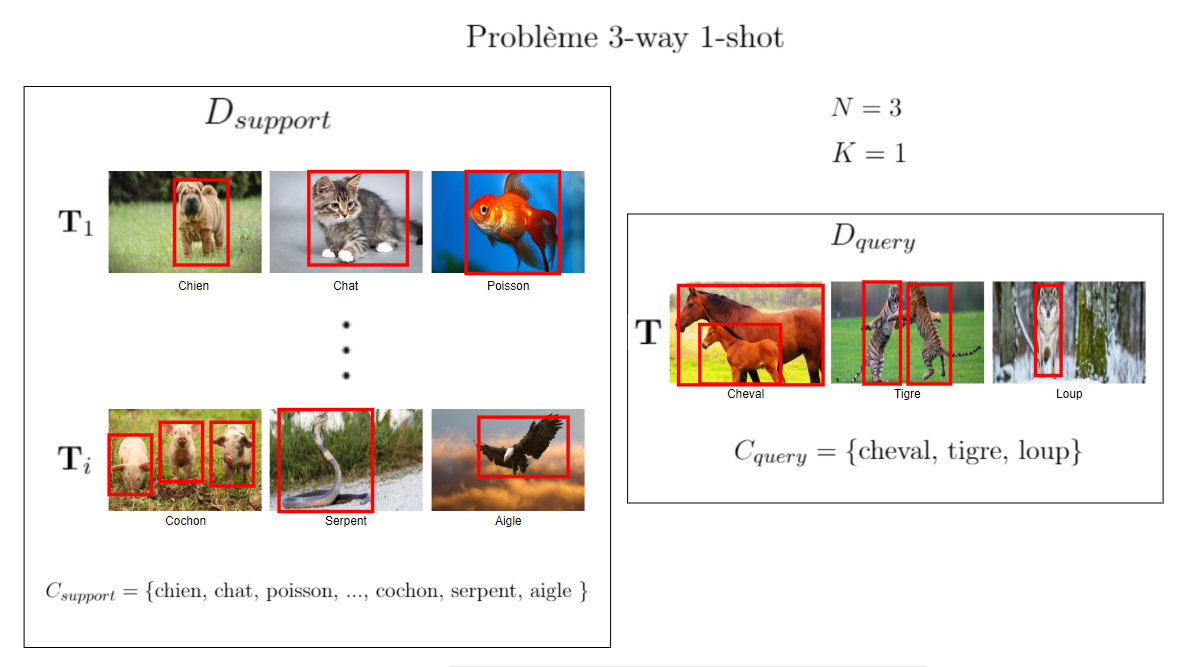
\includegraphics[scale=0.5]{img/Formalisation-FSOD.PNG}
\caption{Exemple de formalisation pour un problème 3-way 1-shot où le but est de détecter des chevaux, tigres et loups en utilisant un dataset de support d'animaux.}
\label{fig:Formalisation-FSOD}
\end{figure}

% Catégorisation solutions
\section{Catégorisation des solutions}
\label{sec:FSOD-categorisation}
Au vu du caractère récent de la recherche sur la FSOD, une catégorisation n'a pas encore été installée dans la communauté. On peut cependant constater qu'il n'existe, pour le moment, que des solutions utilisant le paradigme du meta-learning en FSOD. C'est pourquoi nous faisons le parallèle avec les variantes du paradigme de meta-learning utilisées en few-shot classification\footnote{Voir la section \ref{sec:FSOD-FSL-meta}.} pour définir une séparation plus claire pour la détection.

\subsection{Basé sur le metric learning}
Cette catégorie est la plus populaire à l'heure actuelle. Comme pour la classification, un détecteur basé sur du metric learning va calculer pour chaque image une représentation réduite d'image en vecteur de caractéristiques entre lesquelles on peut calculer une distance. Dans le cas de la détection, ce calcul d'une représentation est faite dans deux buts :
\begin{itemize}
    \item Discriminer les ROI trouvées par le détecteur afin de ne pas être trompé par les objets non-pertinents.
    \item Classifier les ROI restantes selon les $N$ catégories d'objets recherchées.
\end{itemize}

\subsubsection*{Vue d'ensemble de l'architecture}
On entraîne le détecteur sur les tâches $\{\textbf{T}_i\}$. Une tâche $\textbf{T}_i$ est composée de :
\begin{itemize}
    \item $\textbf{S}_i$ : un ensemble de $K$ images de support pour chacune des $N$ catégories que $\textbf{T}_i$ cherche à détecter. On dispose des localisations des objets dans ces images.
    \item $\textbf{V}_i$ : un ensemble de $Q$ images de validation. Une image de validation sert à évaluer la performance du détecteur pour la tâche, c'est-à-dire qu'on mesure la précision des bounding boxes trouvées par le détecteur par rapport à la vérité terrain. Cette évaluation de la détection sera ensuite utilisée pour améliorer les paramètres du réseau pour la prochaine tâche.
\end{itemize}

Le détecteur calcule, pour chaque classe, les vecteurs de caractéristiques sur base des objets localisés dans les images de $\textbf{S}_i$. Ces vecteurs prennent en compte la localisation des objets, afin de pouvoir ensuite discriminer les zones d'intérêt trouvées dans une image de validation.

\begin{figure}[!h]
\centering
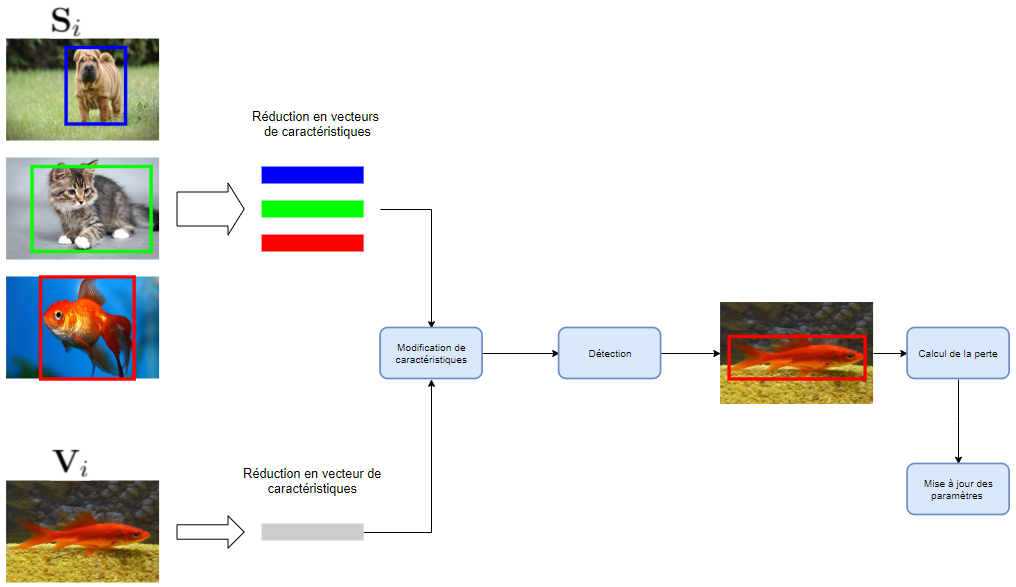
\includegraphics[scale=0.5]{img/DML.PNG}
\caption{Exemple d'entraînement pour une tâche $\textbf{T}_i$ de type 3-way 1-shot avec une seule image de validation pour $\textbf{V}_i$.}
\label{fig:DML}
\end{figure}

Après le calcul des vecteurs de caractéristiques de $\textbf{S}_i$, on évalue la détection grâce aux images de $\textbf{V}_i$. Pour chaque image de $\textbf{V}_i$, on calcule son vecteur des caractéristiques. On modifie celui-ci à l'aide des vecteurs des images de support avec une opération\footnote{Cette "opération" change fortement en fonction des articles. C'est pourquoi nous ne cherchons pas à la détailler ici.} dont le but est d'atténuer les caractéristiques de l'image de validation qui ne sont pas pertinentes et de "surligner" celles qui ont de l'importance par rapport aux objets recherchés. Ensuite, on applique un algorithme de détection propre à la méthode\footnote{Une variante de Faster R-CNN \cite{Faster-R-CNN}, SSD \cite{SSD}, YOLO \cite{YOLO}, etc. Tout dépend de l'algorithme de FSOD utilisé.} avec l'aide du vecteur de caractéristiques modifié par les vecteurs de $\textbf{S}_i$. On calcule ensuite la perte sur les détections trouvées pour l'image de $\textbf{V}_i$. On ré-entraîne l'entièreté du modèle (calcul des vecteurs de caractéristiques, détection, etc) sur base de cette perte. La figure \ref{fig:DML} illustre un résumé de la variante.

Après cette phase d'entraînement, le détecteur est capable de résoudre la tâche cible $\textbf{T}$. Il calcule les vecteurs de caractéristiques pour les $N\times K$ images de la tâche $\textbf{T}$ et est capable d'effectuer une détection pour $\textbf{T}$.


\subsection{Optimisation des paramètres du détecteur}
Cette pratique est moins développée que celle sur le metric-learning, c'est pourquoi nous choisissons de ne pas entrer dans les détails des explications ici. Le but de cette variante est de faire apprendre une optimisation de paramètres au détecteur, qui lui permettra de minimiser la perte le plus rapidement possible pour une nouvelle tâche. 

Les algorithmes de cette catégorie sont habituellement composés de deux composants : le détecteur et le \textit{meta-learner}. Le détecteur a pour rôle de réaliser une détection pour une tâche $\textbf{T}_i$. Le rôle du meta-learner est de créer une bonne adaptation des paramètres de ce détecteur afin que celui-ci soit capable de faire une meilleure détection pour la prochaine tâche.

Lors de l'entraînement, le détecteur apprend en résolvant une tâche $\textbf{T}_i$. Après l'opération de détection, le meta-learner calcule les "meta-info" sur base de la détection faite par le détecteur sur $\textbf{T}_i$. Ces meta-infos servent à faire apprendre au meta-learner à adapter les paramètres $\theta$ du détecteur ainsi que ses meta-paramètres. Pour la tâche suivante $\textbf{T}_{i+1}$, le meta-learner fournit les paramètres $\theta$ et les méta-paramètres optimisés au détecteur afin que celui-ci exécute une meilleure détection.

\hspace{1pt}
\par\noindent\rule{\textwidth}{0.4pt}

Comme nous l'expliquons dans ce chapitre, la FSOD est une problématique récente pour laquelle on recherche encore une solution qui s'impose par rapport aux autres. Nous montrons que le paradigme du meta-learning est actuellement une piste fortement exploitée pour y parvenir et qu'une de ses variantes, le metric learning, semble être la tendance la plus populaire. Les recherches en FSOD ayant débuté récemment, il n'existe pas encore de comparaison entre les algorithmes existants. Nous tentons donc, dans le chapitre \ref{chap:analyse}, de réaliser une comparaison des résultats publiés dans les articles de recherche.

% analyse %
\chapter{Analyse comparative}
\label{chap:analyse}

Le transfer learning et la FSOD sont deux approches qui diffèrent dans leur conception mais qui ont pour même objectif de répondre au besoin de faire face au manque d'images annotées pour l'entraînement d'un détecteur. Dans ce chapitre, nous analysons les résultats présentés par les articles des modèles de détection pour chacune des deux approches afin de tenter d'expliquer l'intérêt de chacune. Nous montrons aussi les limitations de nos analyses.

% Méthodologie %
\section{Informations recherchées}
\label{sec:analyse-metodologie}

%\subsection{Organisation de l'analyse}
%Nous organisons notre analyse des résultats en deux phases :
%\begin{enumerate}
%    \item \textbf{Comparaison propre à l'approche :} pour chaque approche\footnote{C'est-à-dire, transfer learning ou few-shot object detection}, comparer les résultats des différents modèles que nous avons retenus dans notre recherche bibliographique.
%    \item \textbf{Comparaison entre approches:} nous prenons les modèles les plus performants pour le transfer learning et la FSOD et nous comparons les résultats. Nous définissons ensuite les avantages et inconvénients des approches sur base des résultats trouvés.
%\end{enumerate}

%\subsection{Informations recherchées}
%\label{subsec:info-recherchee}
Les informations qui nous intéressent pour comparer les modèles constituant l'état de l'art des deux approches sont : 
\begin{itemize}
    \item La précision du détecteur.
    \item La quantité d'images annotées requise pour obtenir cette détection, qui sert à mesurer l'importance du coût de l'étape d'acquisition d'images annotées.
    \item Le/les dataset(s) utilisé(s) pour la méthode.
    \item Le type de détecteur utilisé pour le modèle (1-stage ou 2-stage). Comme évoqué dans la section \ref{sec:class-vs-detect}, un détecteur de type 1-stage a tendance à être moins précis mais plus rapide qu'un détecteur de type 2-stage. Cette information est importante pour relativiser les résultats en terme de précision.
\end{itemize}


\section{Les solutions de transfer learning}
\label{sec:analyse-transfer-learning}

Comme nous le voyons dans le tableau \ref{tab:generic-table}, les méthodes les plus utilisées dans la littérature sont celles du Deep Learning transfer. C'est, en effet, la méthode qui obtient les meilleurs résultats et s'adapte le mieux à de nombreuses applications.

Parmi les points de comparaison évoqués par le tableau \ref{tab:generic-table} se trouve le nombre d'images dont la base de destination et le score obtenue par le réseau. Le nombre d'image est au moins aussi important que le score car un bon score avec un grand nombre d'image n'est pas toujours pertinent vis à vis de notre objectif. 

Un point important de comparaison qui fait aussi partie de notre tableau est le fait de pouvoir faire des taches de classification ou de régression avec le réseau. Ceci peut être fait avec le Deep Learning mais aussi avec le multi-tasking, ce qui le rend particulièrement intéressant pour les tâches que l'on veut faire. De plus le score obtenu n'est pas calculé de la même manière, celui de la régression est un score \textbf{mAP} et celui de la classification un \textbf{classification accuracy}.

Ces scores peuvent se comparer dans le sens où ils donnent une idée de la fiabilité des résultats du réseau. Il ne reste cependant pas comparable de manière stricte car il ne s'agit pas de la même métrique, le \textbf{mAP} calcul la bonne position de Bounding Box et la \textbf{classification accuracy} le pourcentage de classification réussis.

Ainsi on voit que même si les problèmes de régression ont un nombre d'images par base de données beaucoup plus élevés, le fait qu'ils soient capables de s'attaquer à ce problème spécifique leur permet d'être mis en avant. Malgré son score légèrement supérieur, le plus intéressant des modèles de régression est Mobile Netv2 pour son nombre d'images faibles par rapport à son score.

En classification, il se démarque deux grands réseaux, le JAN et le ResNet50 qui a tous deux moins de 600 images. L'avantage du JAN est d'être un réseau entraîné sur des bases de données classiques (Office31 et ImageCLEF-DA) tandis que le Res Net50 est entraîné sur quelque chose de plus spécifique.

Un biais important des scores est que les travaux sont très spécialisés dans leur domaine et choisissent des données qui mettent en valeur leurs travaux de manière sensible. Ainsi le ResNet50 est très efficace sur la base de 531 images ARCATIT, qui est une base de données d'image de sonar, mais ne sera sûrement pas aussi efficace sur une base représentant autre chose.

\begin{table}[]
\begin{tabular}{ccccc}
\hline
\textbf{Type}                                    & \textbf{Modèle} & \textbf{Dataset(s)} & \textbf{Score (\%)}&  \textbf{tâche}\\ \hline
Deep TL avec adversial & JAN        &  600 images &  84\% & classification\\
Multi-tasking      & Taskonomie     &  150000 img/tch - 26 tâches & 80\% & régression\\
Deep Learning transfer  & MobileNetV2  & 10000 images &   78.29\%   & régression     \\
Deep Learning transfer   & VGG-16 & 6900 images&  99.80\% & classification\\
Deep Learning transfer  & ResNet50 & 531 images&  94\% & classification \\
\end{tabular}
\caption{Table de comparaison de modèle de transfer learning}
\label{tab:generic-table}
\end{table}


\section{Les solutions de few-shot object detection}
\label{sec:analyse-FSOD}
Nous adaptons l'analyse des informations recherchées (mentionnées en section \ref{sec:analyse-metodologie}) au problème de la FSOD pour éviter de perdre de l'intérêt dans notre comparaison. En effet, des informations telle que la quantité d'images annotées requise ne suffisent pas à illustrer la nature d'une tâche $N$-way $K$-shot que tente de résoudre un détecteur en FSOD.

Le tableau \ref{tab:FSOD-table} montre la compilation des observations faites par les articles de recherche sur leurs méthodes de FSOD. Ce sont, à notre connaissance, les seuls articles existants sur le sujet. Dans ce tableau, nous préservons la notion de tâche $N$-way $K$-shot qui nous renseigne implicitement sur le nombre $N \times K$ d'images annotées requises.

Globalement, les résultats présentés sont encore loin de rivaliser avec l'état de l'art en détection d'objets générique, où les détecteurs peuvent atteindre des scores de précision (mAP) de 86.9\% sur Pascal VOC 2007 \cite{SNIPER}, par exemple. Au vu de ce qui a été dit en section \ref{sec:FSOD-verrous}, on sait que la FSOD en est encore à ses débuts. Néanmoins, nous pensons que les résultats sont prometteurs.


% table FSOD
\begin{table}[]
\begin{tabular}{ccccc}
\hline
\textbf{Type}                                    & \textbf{Modèle}                         & \textbf{Dataset(s)}                       & \textbf{Tâche}                                                                                                 & \textbf{mAP (\%)}                                                                                           \\ \hline
{\color[HTML]{333333} }                          & \cellcolor[HTML]{FFCCC9}Meta-RCNN \cite{anonymous2020metarcnn}    & \cellcolor[HTML]{FFCCC9}ImageNet-LOC      & \cellcolor[HTML]{FFCCC9}\begin{tabular}[c]{@{}c@{}}50-way 1-shot\\ 50-way 5-shot\end{tabular}                  & \cellcolor[HTML]{FFCCC9}{\color[HTML]{333333} \textbf{\begin{tabular}[c]{@{}c@{}}25.1\\ 40.3\end{tabular}}} \\
{\color[HTML]{333333} }                          & \cellcolor[HTML]{FFCCC9}RepMet \cite{RepMet}          & \cellcolor[HTML]{FFCCC9}ImageNet-LOC      & \cellcolor[HTML]{FFCCC9}\begin{tabular}[c]{@{}c@{}}50-way 1-shot\\ 50-way 5-shot\\ 50-way 10-shot\end{tabular} & \cellcolor[HTML]{FFCCC9}\begin{tabular}[c]{@{}c@{}}24.1\\ 39.6\\ \textbf{49.2}\end{tabular}                          \\
{\color[HTML]{333333} }                          & Attention-RPN \cite{attention-rpn}                           & FSOD dataset \cite{attention-rpn}                             & \begin{tabular}[c]{@{}c@{}}1-way 5-shot\\ 5-way 5-shot\end{tabular}                                            & \begin{tabular}[c]{@{}c@{}}69.8\\ 61.6\end{tabular}                                                         \\
\multirow{-4}{*}{{\color[HTML]{333333} 2-stage}} & \cellcolor[HTML]{BDF0FF}Meta-RCNN \cite{Meta-RCNN-19}    & \cellcolor[HTML]{BDF0FF}VOC2007 \cite{Pascal-VOC}           & \cellcolor[HTML]{BDF0FF}\begin{tabular}[c]{@{}c@{}}5-way 1-shot\\ 5-way 5-shot\\ 5-way 10-shot\end{tabular}    & \cellcolor[HTML]{BDF0FF}\textbf{\begin{tabular}[c]{@{}c@{}}19.9\\ 45.7\\ 51.5\end{tabular}}                 \\ \hline
                                                 & \cellcolor[HTML]{BDF0FF}Feat. Reweight. \cite{feature-reweighting} & \cellcolor[HTML]{BDF0FF}VOC2007 \cite{Pascal-VOC}           & \cellcolor[HTML]{BDF0FF}\begin{tabular}[c]{@{}c@{}}5-way 1-shot\\ 5-way 5-shot\\ 5-way 10-shot\end{tabular}    & \cellcolor[HTML]{BDF0FF}\begin{tabular}[c]{@{}c@{}}19.2\\ 40.6\\ 47.2\end{tabular}                          \\
\multirow{-2}{*}{1-stage}                        & \cellcolor[HTML]{FFFFFF}Meta-SSD \cite{Meta-SSD}        & \cellcolor[HTML]{FFFFFF}VOC2007 \cite{Pascal-VOC} + VOC2012  & \cellcolor[HTML]{FFFFFF}\begin{tabular}[c]{@{}c@{}}5-way 1-shot\\ 5-way 5-shot\end{tabular}                    & \cellcolor[HTML]{FFFFFF}\begin{tabular}[c]{@{}c@{}}27.3\\ 27.8\end{tabular}                                
\end{tabular}
\caption{Tableau de présentation des modèles de few-shot object detection existants et de leurs résultats en mAP (\%) suivant la tâche sur laquelle ils ont été évalués. Les types de détecteur (1-stage ou 2-stage) sont distingués pour tenir compte de leurs différences (voir la section \ref{sec:class-vs-detect} pour les différences). Les tâches similaires sont regroupées en couleur, pour faciliter la lecture des résultats. les tâches similaires comparées sur ImageNet-LOC sont marquées en \colorbox[HTML]{FFCCC9}{ROUGE}. Les tâches similaires comparées sur VOC2007 \cite{Pascal-VOC} sont marquées en \colorbox[HTML]{BDF0FF}{BLEU}. Les meilleurs résultats en précision pour les tâches similaires sont mis en \textbf{gras}. À ne pas confondre, deux modèles possèdent le même nom dans ce tableau (Meta-RCNN) mais sont bien deux modèles différents.}
\label{tab:FSOD-table}
\end{table}




\subsection*{Biais de comparaisons}
Nous affirmons que le tableau \ref{tab:FSOD-table} est avant tout destiné à montrer une compilation de résultats dans le but de donner une idée au lecteur plutôt qu'une comparaison fiable. Nous définissons plusieurs biais qui empêchent de prendre ce tableau en tant que comparatif.

Premièrement, une des raisons évidentes est la différence des tâches $N$-way $K$-shot présentées. Des tâches différentes reviennent à changer totalement le problème que le détecteur tente de résoudre, en plus de changer la quantité d'images annotées disponibles pour le détecteur. Et, comme la quantité de données annotées est très réduite en FSOD, une différence normalement négligeable d'une seule image devient tout de suite très importante.

Deuxièmement, l'autre raison évidente est la différence de dataset utilisé pour certains détecteur. À l'instar d'une différence de tâches, la comparaison de deux résultats basés sur deux datasets différents reviendraient à comparer deux problèmes qui n'ont pas de rapport entre eux. En plus de cela, il faut ajouter le fait que les images présentes dans ces datasets peuvent varier en difficulté\footnote{Par exemple, une image présentant plusieurs objets recherchés dans un environnement encombrés d'objets non-pertinents est plus "difficile" qu'une image avec un seul objet recherché en avant plan sur un fond uni.}, ce qui peut influer sur les performances observées.

Troisièmement, on voit que certains modèles se comparent sur base des mêmes tâches avec le/les même(s) dataset(s). La comparaison paraîtrait pertinente mais nous émettons quand même une réserve pour ce cas de figure. La plupart des tests rencontrés dans les articles sélectionnent les $N \times K$ images de la tâche au hasard dans un dataset de grande de taille. Dans une situation comme en FSOD où le nombre d'images annotées disponibles à l'entraînement est très réduit, la sélection aléatoire d'une image plus "compliquée" (arrière plan encombré d'objets non-pertinents, par exemple) que les autres peut avoir une influence non désirée sur le mAP. 

Pour une comparaison réellement équitable, nous avançons qu'il est préférable de maintenir aussi les mêmes échantillons de tâches originaires du même dataset à travers tous les détecteurs.

\section{Comparaison entre approches}
\label{sec:analyse-comparaison}
En se basant sur l'apparence générale des résultats obtenus pour le transfer learning (tableau \ref{tab:generic-table}) et pour la FSOD (tableau \ref{tab:FSOD-table}), on remarque que le transfer learning a tendance à être plus précis en terme de mAP mais à demander beaucoup plus d'images annotées.

On émet l'hypothèse que les deux approches essayent de traiter un cas de manque de données annotées différent :
\begin{itemize}
    \item Pour le transfer learning, on dispose d'un nombre d'images annotées réduit mais toujours conséquent et on transfère la connaissance d'un modèle déjà entraîné au détecteur en transfer learning pour que celui-ci converge plus vite avec les données réduites.
    
    \item Pour la few-shot object detection, on recherche à exécuter une détection dans des cas de figure où on dispose d'un nombre d'images annotées extrêmement réduit (de 1 à 10 images). Pour ce faire, on construit un savoir antérieur à partir d'un entraînement sur des images provenant de datasets déjà existants, puis on adapte ce savoir antérieur à la tâche cible à données réduites.
\end{itemize}

On ne peut cependant pas, avec les tableaux de comparaison obtenus, montrer l'efficacité d'une méthode de manière pertinente puisqu'on ne compare pas les mêmes tâches. Dans le cas où on voudrait tout de même faire une comparaison des deux approches, il existe toujours le problème de définir une base de comparaison fiable sur lesquelles nous appuyer. En effet, à notre connaissance, il n'existe pas de méthodologie permettant de comparer les deux approches de manière équitable. Si nous nous basons sur une configuration comme pour la FSOD, celle-ci est avantagée par rapport au transfer learning et vice-versa. Il existe donc un besoin pour notre projet de définir une méthodologie de comparaison équitable entre le transfer learning et la few-shot object detection.


\par\noindent\rule{\textwidth}{0.4pt}

Notre analyse des résultats permet de dégager certaines tendances dans les détecteurs pour chaque approche. Nous montrons également les problèmes qu'il y a dans l'analyse des résultats des détecteurs pour le transfer learning ou la FSOD, ainsi que les défis à relever pour comparer les deux approches entre elles. Tout cela amène à la nécessité de produire, premièrement, des tests comparatifs montrant les performances des algorithmes spécifiques à une approche, et deuxièmement, de mettre au point une méthodologie la plus fiable possible pour comparer les approches entre elles.

% Mise en pratique future
\chapter{Mise en pratique future}
\label{chap:future-works}
Dans nos analyses au chapitre \ref{chap:analyse}, nous montrons le besoin d'effectuer des tests comparatifs pour corriger les biais trouvés sur les résultats observés. Nous montrons aussi la nécessité de mettre en place une méthodologie de comparaison équitable entre la FSOD et le TL afin d'expérimenter et comprendre les avantages et les inconvénients des deux approches. Dans ce chapitre, nous décrivons les travaux que nous ferons pour la suite du projet, dont le but sera de répondre aux besoins évoqués.

% Base de comparaison des
\section{Mise au point d'une base de comparaison}
Pour notre travail de comparaison, nous décidons de sélectionner les algorithmes de détection dont le code est fourni par les rédacteurs des articles trouvés pendant notre bibliographie. Cela nous permet de nous concentrer sur l'analyse et la comparaison des résultats fournis par ces détecteurs. Dans le cas où une implémentation venait à manquer pour un détecteur particulièrement intéressant, nous essayerons de la fournir.

\subsection{Comparaison "intra-approche"}
Pour obtenir une analyse pertinente des résultats des détecteurs d'une même approche (FSOD ou TL), nous devons effectuer des tests sur les mêmes tâches et les mêmes données, afin d'être sûr de limiter les biais de comparaisons. Cela se traduit, de manière générale, par l'utilisation des mêmes datasets et la définition du même problème de détection à résoudre. Spécifiquement, pour la FSOD, il faut également assurer une sélection des tâches $N$-way $K$-shot équitable pour éviter le biais de la difficulté des images variable qui influence la performance. % TODO ?

\subsection{Comparaison "inter-approches"}
Notre travail consistera désormais à tester certaines méthodes de transfer learning et de few-shot object detection. Dans ce cas, la difficulté est de comparer efficacement les deux approches au vu de la métrique intrinsèque à chacune des approches. Nous nous effectuerons des tests sur des bases de données identiques. Nous essayerons de mettre au point une méthodologie qui permet de réaliser une comparaison équitable, c'est-à-dire qui n'avantage pas l'apprentissage ou la détection d'un détecteur d'une approche par rapport à l'autre.

%Le transfer learning étant vaste et le few-shot en étant un cas particulier, il faut nous concentrer sur un cas particulier du TL. Un cas intéressant est le multi-tasking learning permettant de faire l'apprentissage de plusieurs taches en simultanée. La base de données d'image est ici fourni en plus du code.

%De même nous pourrons tester un réseau de Deep transfère Learning avec les JAN (joint Adaptation Networks) qui va permettre de travailler sur des base de données plus communes du type ImageNet ou Office-31.

\section{Interface de simulation de détections}
En parallèle de notre travail d'analyse, nous proposerons une vue de notre travail au moyen d'une interface permettant de simuler des détections avec les algorithmes que nous avons utilisé dans notre travail de comparaison. Le but de cette interface est de fournir à un utilisateur une vue concrète des performances des détecteurs en transfer learning et en few-shot object detection. La figure \ref{fig:UML_INTERFACE} illustre les fonctionnalités de l'interface.
\begin{figure}[!h]
\centering
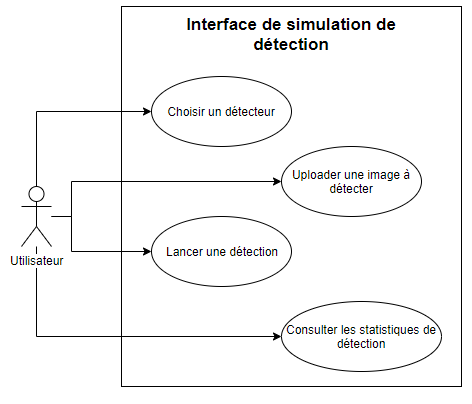
\includegraphics[scale=0.5]{img/UML_INTERFACE.PNG}
\caption{Diagramme UML présentant les fonctionnalités de l'interface de simulation de détections à réaliser.}
\label{fig:UML_INTERFACE}
\end{figure}

%Ensuite nous proposerons une vue de notre travail avec une démonstration qui permettra de voir des comparaisons de plusieurs réseaux. Nous espérons ainsi laisser l'utilisateur pouvoir choisir entre des réseaux non entraînés avec des méthodes de TL et des réseaux de TL et lui laisser voir que les méthodes de TL fonctionnent mieux sur des vidéos contenants plusieurs objets.

%De même afin que l'utilisateur puisse constater ça de lui-même, l'utilisateur pourrait tester le réseau grâce à la webcam du PC de démo.

% Conclusion %
\SpecialSection{Conclusion}

Lors de ces derniers mois, nous avons pu voir de nombreux articles dont le but est de réduire le nombre de données nécessaire à l'entraînement efficace d'un réseau de neurones dans le cadre de la détection d'objets. De nombreux axes et de manières de faire se sont dégagées. Les articles portaient tout d'abord sur le large thème du transfer learning.

Nous avons pu constater des approches spécialisées sur des problèmes particuliers. Nous avons rapidement pu trouver des moyens de sélectionner des articles plus pertinents, que ce soit par rapport à leur résultat en terme de précision ou par rapport à la quantité d'images annotées à fournir.

C'est dans cette optique que nous avons décidé de concentrer une partie de nos efforts sur une approche particulière pour faire face au manque de données : le few-shot learning. Ce domaine permet déjà de faire de la classification sur des bases de données qui contiennent très peu d'images (de 1 à 10 par catégorie d'objets), ce qui correspond parfaitement à nos attentes. Cependant, le few-shot learning appliqué à la détection d'objets ne donne pas encore de résultats convaincants. On peut espérer cependant des progrès pour les années à venir, étant donné que le domaine n'a été exploré que très récemment.

En parallèle, nous nous sommes aussi concentrés sur d'autres manière de faire de la TL qui permettent de faire de la régression de manière efficace. Nous avons sélectionné les domaines de multi-task leaning et de Deep Learning avec adversial qui obtiennent des très bons résultats même si le nombre d'images nécessaire au bon entraînement est finalement supérieur au few-shot learning.

Nous continuerons maintenant notre travail sur la comparaison entre des méthodes de TL et de few-shot qui nous permettront de déterminer de manière expérimentale sur quels cas il est avantageux d'appliquer une méthode plutôt qu'une autre.

\bibliographystyle{myunsrt}
\small
\bibliography{biblio}


\end{document}
